In this section, we analyze the relationship between the excess returns of individual stocks and those of the sector market
using scatter plots.
The objective is to explore whether linear relationships exist, as assumed by the CAPM model. 
Scatter plots are used to visually assess the correlation between variables and to identify potential deviations.
Particular focus is given to outliers and non-linear trends, as these could suggest the need for deeper analysis or
alternative approaches.
The scatter plots reveal a clear relationship between the excess returns of most stocks and the sector market.
For instance, stocks like Johnson \& Johnson, Pfizer, and Medtronic show a well-defined linear trend, indicating a strong 
correlation with market returns. 

\begin{table}[htbp]
    \centering
    \footnotesize
    \renewcommand{\arraystretch}{1.2} % Adjust row height
    \begin{tabular}{|l|c|c|c|c|c|c|c|}
        \hline
        \rowcolor{unired!30} \textbf{Company} & \textbf{$\alpha$} & \textbf{$\beta$} & \textbf{$R^2$} & \textbf{Err. $\alpha$} & \textbf{Err. $\beta$} & \textbf{$\Delta \beta$ [0.025]} & \textbf{$\Delta \beta$ [0.975]} \\ \hline
        Johnson \& Johnson & 0.2451 & 0.7474 & 0.455 & 0.212 & 0.048 & 0.652 & 0.843 \\ \hline
        \rowcolor{gray!10} Boston Scientific & 0.3464 & 0.9036 & 0.207 & 0.458 & 0.105 & 0.698 & 1.109 \\ \hline
        Eli Lilly & 0.5655 & 0.9314 & 0.342 & 0.335 & 0.076 & 0.781 & 1.082 \\ \hline
        \rowcolor{gray!10} Pfizer & -0.3246 & 0.9595 & 0.451 & 0.274 & 0.063 & 0.836 & 1.083 \\ \hline
        Teleflex & 0.3055 & 0.9621 & 0.297 & 0.383 & 0.088 & 0.790 & 1.134 \\ \hline
        \rowcolor{gray!10} Cigna & 0.2511 & 1.0512 & 0.212 & 0.525 & 0.120 & 0.815 & 1.287 \\ \hline
        Revvity & -0.2457 & 1.2225 & 0.265 & 0.527 & 0.120 & 0.985 & 1.460 \\ \hline
        \rowcolor{gray!10} Medtronic & -0.1108 & 0.8613 & 0.384 & 0.282 & 0.065 & 0.734 & 0.988 \\ \hline
        LabCorp Holdings & 0.2675 & 0.9163 & 0.233 & 0.430 & 0.098 & 0.723 & 1.110 \\ \hline
        \rowcolor{gray!10} Humana & 0.5939 & 1.0700 & 0.231 & 0.506 & 0.116 & 0.843 & 1.298 \\ \hline
    \end{tabular}
    \caption{Regression results for each company, detailing Alpha, Beta, R-squared, and confidence intervals.}
    \label{tab:regression_results}
\end{table}

These results suggest that the CAPM model can effectively describe the variability in returns for these stocks, supported by
significant $\beta$ coefficients and high $R^2$ values.
However, some stocks, such as Boston Scientific and Cigna, display more scattered data points around the trendline, 
pointing to weaker correlations and the influence of unique factors that the CAPM might not capture.
In addition, outliers observed in stocks like Revvity and Labcorp Holdings could reflect extraordinary events, such as 
regulatory changes or R\&D results, which may reduce the model s effectiveness for these cases.
The slope of the trendline offers further insights: for example, Eli Lilly and Teleflex demonstrate steeper slopes,
suggesting a high $\beta$ and greater sensitivity to market movements, while flatter slopes, as observed in Humana, indicate
lower exposure to systematic risk.
Overall, our observations suggest that the CAPM model effectively explains the behavior of most stocks analyzed. 
However, instances of high dispersion or the presence of significant outliers underscore the need for further evaluation, 
which will be undertaken in subsequent stages of the analysis.

\begin{figure}[h]
    \centering
    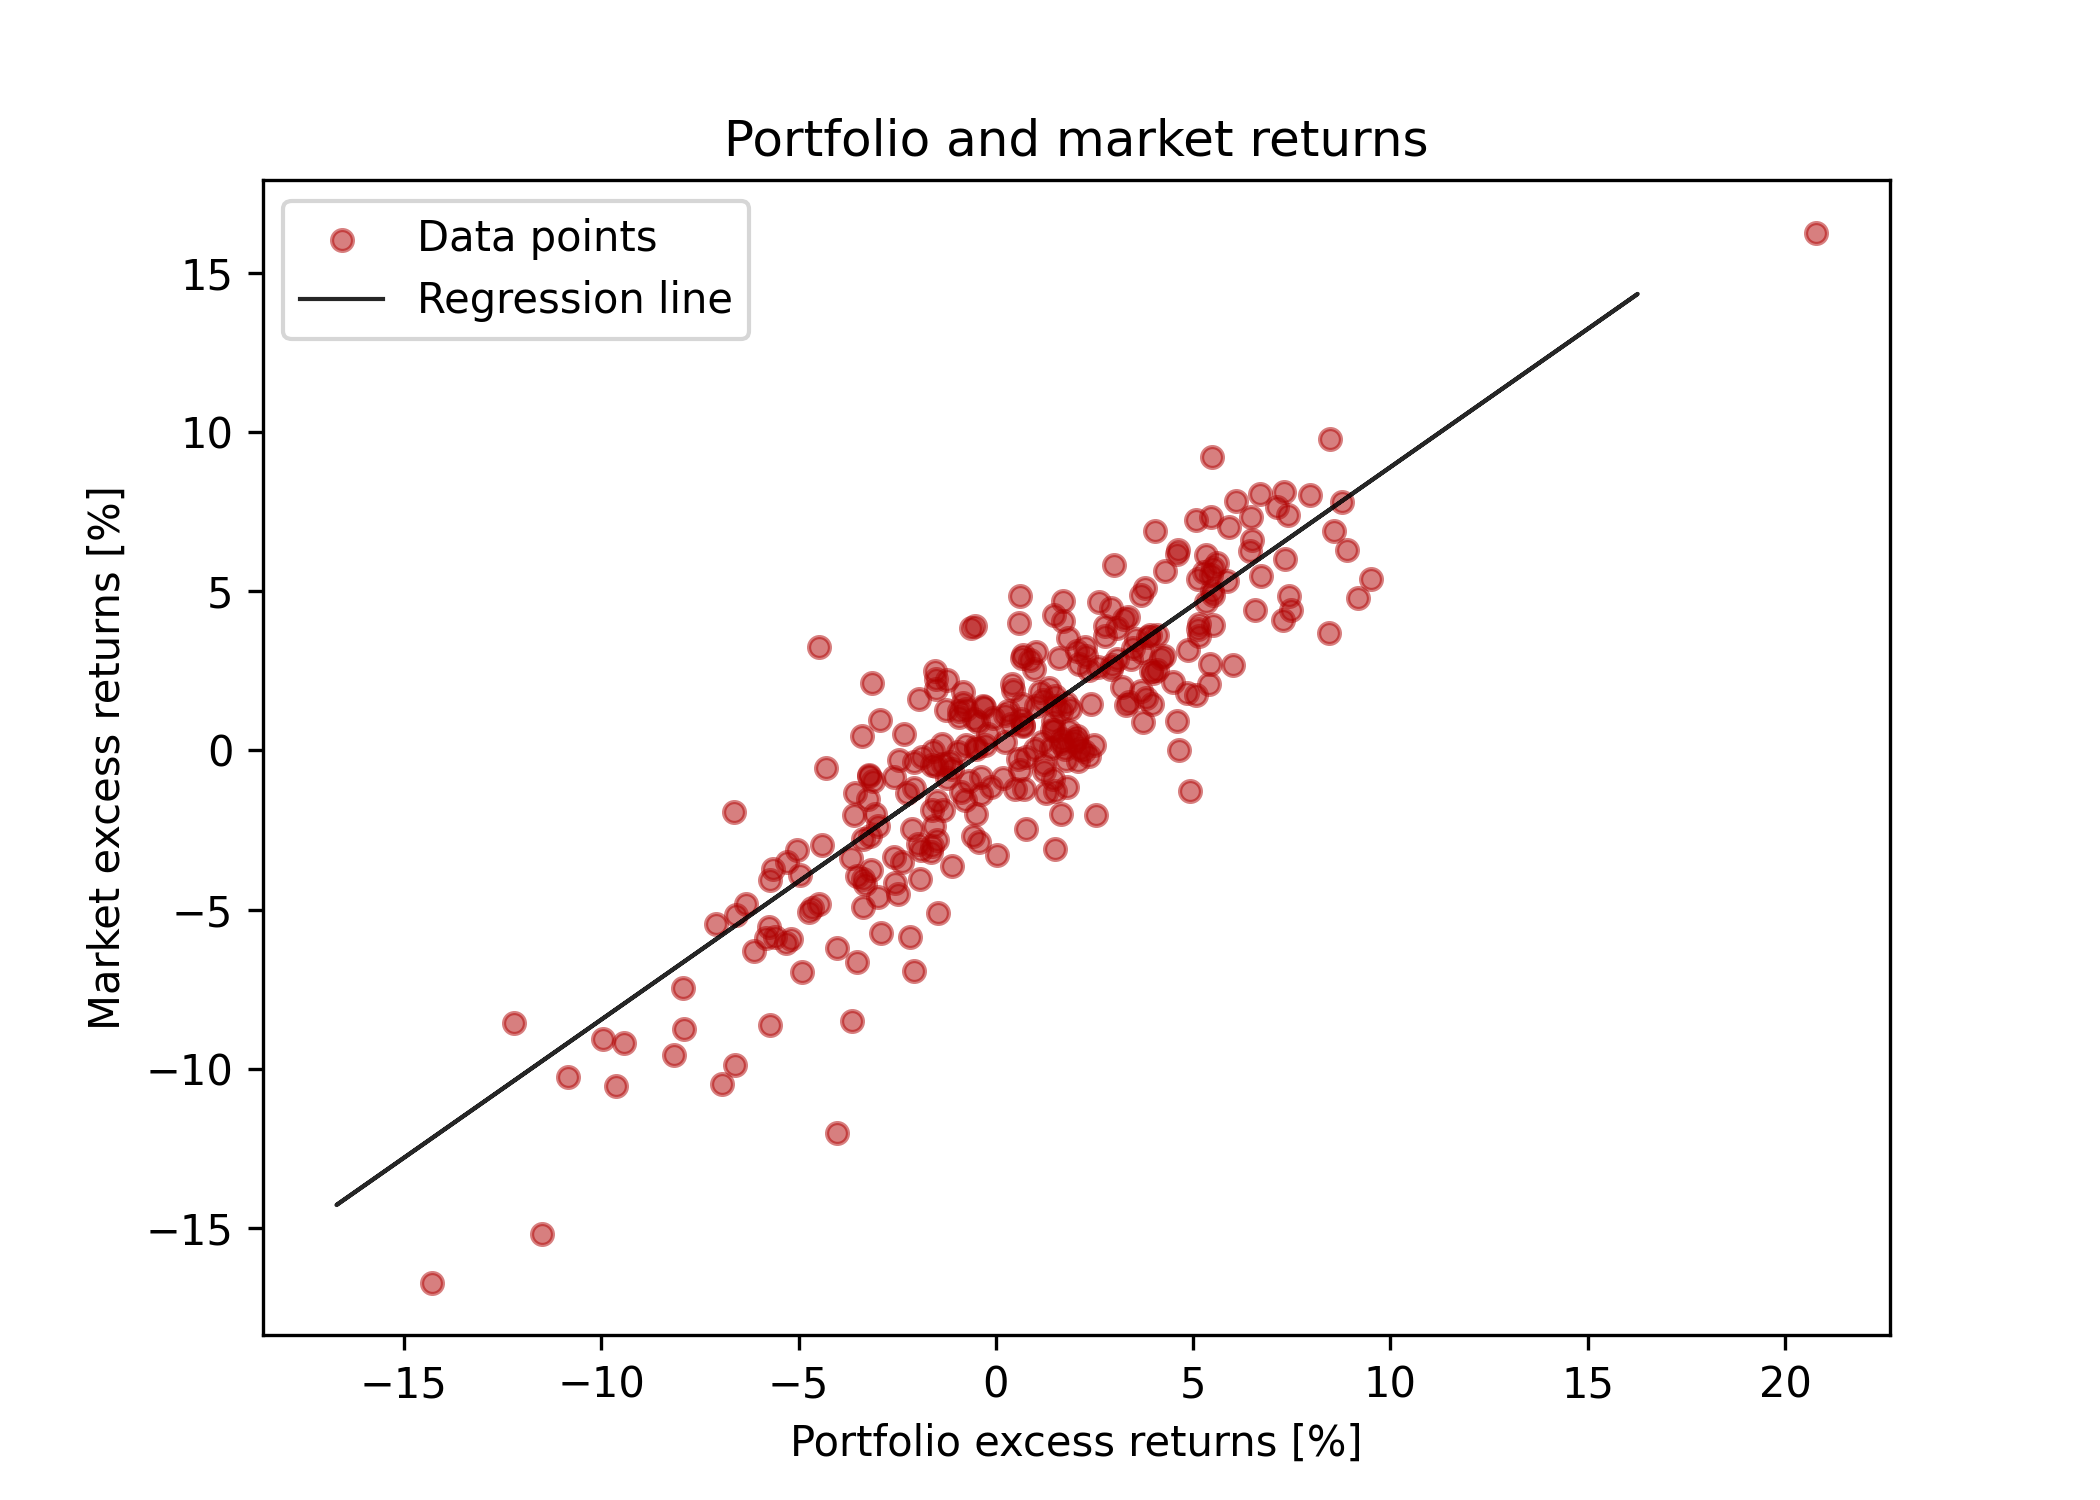
\includegraphics[width=0.8\textwidth]{images/portfolio_regression.png}
    \caption{Scatterplot of portfolio's returns against excess market returns, with linear regression.}\label{fig:portfolio_regression}
\end{figure}